%
%
\documentclass{article}
\usepackage{amsmath}
\usepackage{graphicx}
\usepackage{color}
\usepackage{caption}
\usepackage{amsfonts}
\usepackage[margin=3cm]{geometry}
\usepackage{tikz}
\newcommand{\cE}{\mathcal{E}}                               %

\begin{document}

\title{Small toughness solution}
\author{Tim Large, Dominic Skinner}
\maketitle
\section{Setup}
Recall we have a system goverened by the equations
\begin{equation} \left( \begin{array}{c} p(z) \\ 0 \end{array} \right) =
\int_0^{\infty} \left( \begin{array}{cc} K_{11}(x-z) & K_{12}(x-z) \\
 K_{21}(x-z) & K_{22}(x-z) \end{array} \right)
 \left( \begin{array}{c} g'(x) \\ h'(x) \end{array} \right) dx
\end{equation}
\begin{equation}
p(z) = - \int_z^{\infty} \frac{\lambda}{h(x)^2} dx
\end{equation}
where the kernel terms are given by
\[ \begin{array}{lcl}
\displaystyle K_{11}(z) = \frac{32-24z^2}{(z^2+4)^3} & &
\displaystyle K_{12}(z) = \frac{48z^2-64}{z(z^2+4)^3} \\[19pt]
\displaystyle K_{21}(z) = -\frac{(16z^3+16z^2+4)}{z(z^2+4)^3} & &
\displaystyle K_{22}(z) = -\frac{(32-24z^2)}{(z^2+4)^3} 
\end{array} \] 
with boundary conditions at infinity
\[ h''(x) \to 1, \quad g'(x) \to \frac{1}{2} \]
For a given speed parameter $\lambda$, we wish to find the material toughness
$K$, which is given by
\[ K(\lambda) = \lim_{x\to 0} 3 \sqrt{2\pi} \sqrt{x} \;h'(x) \]
We are interested in the value $\lambda = \lambda_0$ for which 
$K(\lambda_0)=0$, since this is then the propagation speed of a zero-toughness
system. We are also interested in $\lambda \approx \lambda_0$.
%
\section{Zero toughness solution}
% 
Consider setting $K=0$. We investigate only the nature of the solution near
$x=0$. We suspect, (and will verify later) that $p$ is singular near the crack
tip. Thus in equation 1, we can neglect terms that are non singular. 
\[ p(z) = \int_0^{\infty} \frac{h'(x)}{x-z} dx \]
Also have that $p' = \lambda/h^2$. We try the ansatz $h \sim x^{\alpha}$. From
our two equations linking $h$ and $p$, this gives that
\[ p \sim x^{\alpha-1} \]
\[ p' \sim x^{-2\alpha} \]
and so $\alpha = 2/3$. We have made use of the integral
\[ \int_0^\infty \frac{z^{s-1}}{z-x}dz = -\pi \cot (\pi s)z^{s-1} \]
So starting with a solution $h_0 = A_0 x^{2/3} + o(x^{2/3})$ near the
crack tip, we get $\displaystyle p_0(x) = -\frac{3\lambda_0}{A_0^2}x^{-1/3} 
+ O(1)$. Putting this into the lubrication equation $p' h^2 = \lambda_0$, 
we find that 
\[ A_0 = \left( \frac{243 \lambda_0}{4\pi^2} \right)^{1/6} \]
{\color{red}We also can take $g_0 = Bx^{1/2}+\dots$ for $x\to0$. $B$ can only
be found numerically. (N.B. in red since this isn't an issue in \cite{GandD},
and I'm not sure where this came from or if it's even needed.)}
To recap the zero tougness solution takes the form
\begin{alignat*}{2}
h_0(x) &= A_0 x^{2/3} &+ \dots \\
p_0(x) &= -\frac{3\lambda_0}{A_0^2} x^{-1/3} &+ \dots \\
g_0(x) &= Bx^{1/2} &+ \dots 
\end{alignat*}
This holds only when $K=0$ exactly, and the above is a good approximation
for small $x$, all the way to $x=0$.
%
\section{Small toughness solution}
Now let us consider $K>0$ but take $K$ arbitrarily small. One expects for 
$K$ small, that the new solution will look much like the $K=0$ solution.
However for any small, but non-zero, value of $K$, we must have that
$h(x) \sim \frac{2K}{3\sqrt{2\pi}}x^{1/2}$ as $x\to0$. Thus the zero toughness
solution cannot be a good approximation for the entire domain. This is 
resolved by a LEFM boundary layer, following \cite{GandD}.
Outside this boundary layer, we expect behaviour close to the lubrication 
solution. So outside the boundary layer, look for a solution
\begin{align*}
g(x) &= g_0(x) + \cE(K)g_1(x)+o(\cE) \\
h(x) &= h_0(x) + \cE(K)h_1(x)+o(\cE) \\
p(x) &= p_0(x) + \cE(K)p_1(x)+o(\cE) \\
\lambda &= \lambda_0 + \cE(K)\lambda_1+o(\cE) 
\end{align*}
Where $\cE(K)$ is an unknown function of $K$ which will be determined.
We work with $K$ small enough such that $\cE(K) \ll 1$, (will be easily
verified later).
\\
\\
It is important to remember that the above only holds outside the LEFM boundary
layer. To find $\cE$, we will take the outer asymptotics of the LEFM boundary
layer and attempt to match that with the inner asypmtotics of the above 
solution.

\begin{figure}[!ht]\centering
\caption{Matching outer asymptotics of the LEFM boundary later with the inner
asymptotics of the Lubrication region}
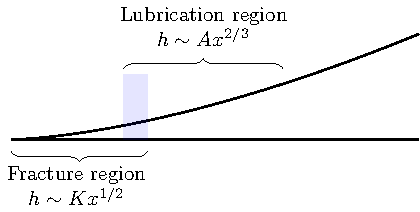
\includegraphics{Fig6.pdf}
\end{figure}


%
% References/Bibliography ////////////////////////////////////////////////////
%
\clearpage 
\begin{thebibliography}{9}  
%
\bibitem{GandD}
Garagash, D.I., Detournay, E.,
\emph{Plane-Strain Propagation of a Fluid-Driven Fracture: Small Toughness
Solution,}
Journal of Applied Mechanics,
2005.
%
%
\end{thebibliography}
\end{document}

